\documentclass{scrartcl}
\usepackage{physics}   % Matrixes and Dirac-notation
\usepackage{amsmath}   % Binear equations
\usepackage{booktabs}  % Tabs
\usepackage{graphicx}  % Pictures/figures
\usepackage{listings}  % Source code
\usepackage{color}     % Colors
\usepackage{mdframed}  % Frames
\usepackage{hyperref}  % Hyperlinks

\definecolor{dkgreen}{rgb}{0,0.6,0}
\definecolor{gray}{rgb}{0.5,0.5,0.5}
\definecolor{mauve}{rgb}{0.58,0,0.82}

%Defining source code
\lstset{frame=tb,
  language=Python,
  aboveskip=3mm,
  belowskip=3mm,
  showstringspaces=false,
  columns=flexible,
  basicstyle={\small\ttfamily},
  numbers=none,
  numberstyle=\tiny\color{gray},
  keywordstyle=\color{blue},
  commentstyle=\color{dkgreen},
  stringstyle=\color{mauve},
  breaklines=true,
  breakatwhitespace=true,
  tabsize=3
}
\makeatletter
\renewcommand*\env@matrix[1][*\c@MaxMatrixCols c]{%
  \hskip -\arraycolsep
  \let\@ifnextchar\new@ifnextchar
  \array{#1}}
\makeatother
\begin{document}
\begin{titlepage}
	\centering
	{\scshape\LARGE $\star$  \par}
	\vspace{4cm}
	{\scshape\huge FYS3150 - Computational Physics  \par}
	\vspace{1cm}
	{\scshape\Large Project 1\par}
	\vspace{2cm}
	{\Large\itshape Even Marius Nordhagen\par}
	\vfill
	{\large \today\par}
\end{titlepage}
\newpage
\begin{abstract}
\subsection*{Abstract}
In this project we are finding the second derivative for a function by the 3-point formula and numerical methods, counting the number of floating point operation (FLOPS) and taking the GPU time for each of the methods. The result was that LU decomposition generated most FLOPS and had longest running time compared with Gaussian elimination, as expected.
\end{abstract}%\vspace{3mm}

\par Source files:
\par \url{https://github.com/evennordhagen/FYS3150/tree/master/Projects/Project1}

\section{Introduction}
When solving mathematical and scientific problems, we are often ending up with differential equations. One example of this is Poisson's equation from electromagnetism;
$$\frac{d^2\phi}{dr^2}=-4\pi r\rho(r)\quad(one\,\,dimension)$$
which was first expressed by Sim\'{e}on Denis Poisson in the 19. century. To solve this, the mathematicians had to find robust methods for solving that kind of equations analytical, with for example the 3-point formula. \par\vspace{2mm} In this project we are starting with the same problem as these mathematicians, but we are going to find numerical solutions to the problem when we already know the analytical solution. We are given a specific source function $f(x)=100e^{-10x}$, and will solve this with numerical methods built on the 3-point formula and linear algebra. The exact solution is given by $u(x)=1-(1-e^{-10})x-e^{-10}$, so in the end we will compare the approach solutions with the exact, and see how good our numerical methods are.

\section{Theory}
In this project we are dealing with a second-order differential equation on the form 
$$\frac{d^2y}{dx^2}+g(x)y=f(x)$$
This can be handy when we are working with Poisson's equation, but there is also many other situations where the solution is handy.
In the lectures we have derived the 3-point formula from forward and backward Euler. The formula is as follows:
$$\frac{d^2u(x)}{dx^2}=\frac{u(x+h)-2u(x)+u(x-h)}{h^2}+{\cal O}(h^2)$$
The last term is the truncation error and $u(x)$ is the function we want to find the second derivative to. We will not include the truncation error in the calculations, but do not forget it, we will come back to it in the results! \par\vspace{3mm}
To short down the calculations I will introduce a simpler notation style, by stating
$$u(x+h)=u_{i+1},\quad u(x)=u_{i},\quad u(x-h)=u_{i-1}$$
And so on. This notation is also closer to that we are using in the programs, but that is important to remember that $i$ has to increase with the same step length $h$ every time we are running a loop, where $h$ has to be chosen. The expression we should solve is therefore:
$$u_{i+1}-2u_i+u_{i-1}=\frac{f_i}{h^2}\equiv d_i$$
where  $i=0,1,...,N-1$ and $N=\frac{1}{h}-1$ since we just are looking at the interval $x\in [0,1]$ (here I enumerate $i$ just like I am going to enumerate it in the scripts).
If we omit the end points (which are uninteresting anyway), we can form a matrix that corresponds to the formula:
$$\mqty(-2&1&0&0&\hdots&0\\
		1&-2&1&0&\hdots&0\\
		0&1&-2&1&\hdots&0\\
		\vdots&\vdots&\ddots&\ddots&\ddots&\vdots\\
		0&0&\hdots&1&-2&1\\
		0&0&\hdots&0&1&-2)
  \mqty(u_1\\u_2\\u_3\\ \vdots\\u_{n-1}\\u_n)=
  \mqty(d_1\\d_2\\d_3\\ \vdots\\d_{n-1}\\d_n)$$
So we have a matrix equation where we know the matrix and the vector $\hat{d}$ (it is just values from our arbitrary function divided by $h^2$), so it should be possible to solve. Maybe you are thinking "Why can we not just find the inverse of A, and multiply on both sides?" This is possible for small matrices, but since the classic way to compute the inverse involves $n^2$ number of FLOPS, this is very slow for big matrices if it is even possible. In our case the matrix only has elements on its diagonal and on the both sides of the diagonal, so the matrix is tridiagonal. We are going to study two methods to solve this problem numerical, but first we need the theory behind the methods:
		
\subsection{Method 1 - Gaussian elimination}
The first method I will take a closer look at, is the Gaussian elimination, which is a simple, well-known linear algebraic method. The thought behind the elimination is to transform the matrix into the identity matrix ($I$) by forward and backward substitution, and then $\hat{u}$ will be equal to the vector on the right side, which I will call $\hat{\tilde{d}}$. Mathematical it will looks like:
$$I\hat{u}=\hat{\tilde{d}}$$
This is just the idea, how is the elimination?
The first thing I want to do, is to replace the matrix with a general tridiagonal matrix. This does not only makes the elimination more general, it also makes the calculations a lot more transparent. The method works for a $n\times n$ matrix where $n$ is an arbitrary integer, but I will show it with a $4\times4$ matrix just to short down the calculations. So the starting point is
$$\mqty(a_1&b_1&0&0\\
		c_1&a_2&b_2&0\\
		0&c_2&a_3&b_3\\
		0&0&c_3&a_4)
\mqty(u_1\\u_2\\u_3\\u_4)=\mqty(d_1\\d_2\\d_3\\d_4)$$
\subsubsection{Forward substitution}
In this part we want to remove the elements under the diagonal by row operations. 
From linear algebra we know that we can do this by row reducing the extended matrix
\[
 \left(
  \begin{array}{cccc|c}
   a_1 & b_1 & 0 & 0 & d_1 \\
   c_1 & a_2 & b_2 & 0 & d_2 \\
   0 & c_2 & a_3 & b_3 & d_3 \\
   0 & 0 & c_3 & a_4 & d_4 \\
  \end{array}
 \right)\sim
 \left(
  \begin{array}{cccc|c}
   a_1 & b_1 & 0 & 0 & d_1 \\
   0 & a_2-\frac{c_1b_1}{a_1} & b_2 & 0 & d_2-\frac{d_1c_1}{a_1} \\
   0 & c_2 & a_3 & b_3 & d_3 \\
   0 & 0 & c_3 & a_4 & d_4 \\
  \end{array}
 \right)
\]
Here I have used the row operation $II-\frac{c_1}{a_1}I$ (where the roman numbers enumerate the rows from the top). Already now we can see that the final matrix is going to be pretty ugly, so I will introduce two new variables that is defined by
\begin{equation}
\tilde{a}_i=a_i-\frac{b_{i-1}c_{i-1}}{\tilde{a}_{i-1}}
\end{equation}
\begin{equation}
\tilde{d}_i=d_i-\frac{\tilde{d}_{i-1} c_{i-1}}{ \tilde{a}_{i-1}}
\end{equation}
Now we can count the number of FLOPS as a function of $n$. Each of the equations above (equation (1) and (2)) generates $3n$ FLOPS when we are running it for an array with $n$ elements.  With doing this we also get a much more aesthetic matrix, and by continue where we stopped above, we will end up with the matrix
\[
 \left(
  \begin{array}{cccc|c}
   a_1 & b_1 & 0 & 0 & d_1 \\
   0 & \tilde{a}_2 & b_2 & 0 & \tilde{d}_2 \\
   0 & 0 & \tilde{a}_3 & b_3 & \tilde{d}_3 \\
   0 & 0 & 0 & \tilde{a}_4 & \tilde{d}_4 \\
  \end{array}
 \right)
\]
We can write the equation as
$$\mqty(\tilde{a}_1 & b_1 & 0 & 0 \\
		0 & \tilde{a}_2 & b_2 & 0 \\
		0 & 0 & \tilde{a}_3 & b_3 \\
		0 & 0 & 0 & \tilde{a}_4)
  \mqty(u_1 \\ u_2 \\ u_3 \\ u_4)=
  \mqty(\tilde{d}_1 \\ \tilde{d}_2 \\ 
  		\tilde{d}_3 \\ \tilde{d}_4)$$
with the boundary conditions 
\begin{equation*}
\tilde{a}_1=a_1,\quad \tilde{d}_1=d_1 
\end{equation*}

\subsubsection{Backward substitution}
Here we are going to remove the elements above the diagonal, and it is called backward substitution. The row operations are much the same as for the forward substitution, but we start with the element of highest index and go to the left. To remove $b_3$ we need to do the row operation $III-\frac{b_3}{\tilde{a}_4}IV$, which gives us
\[
 \left(
  \begin{array}{cccc|c}
   \tilde{a}_1 & b_1 & 0 & 0 & \tilde{d}_1 \\
   0 & \tilde{a}_2 & b_2 & 0 & \tilde{d}_2 \\
   0 & 0 & \tilde{a}_3 & b_3 & \tilde{d}_3 \\
   0 & 0 & 0 & \tilde{a}_4 & \tilde{d}_4 \\
  \end{array}
 \right)\sim
 \left(
  \begin{array}{cccc|c}
   \tilde{a}_1 & b_1 & 0 & 0 & \tilde{d}_1 \\
   0 & \tilde{a}_2 & b_2 & 0 & \tilde{d}_2 \\
   0 & 0 & \tilde{a}_3 & 0 & \tilde{d}_3-\frac{b_3\tilde{d}_4}{\tilde{a}_4} \\
   0 & 0 & 0 & \tilde{a}_4 & \tilde{d}_4 \\
  \end{array}
 \right)
\]
 
The principle is exactly the same for the next two elements ($b_2$ and $b_1$), and after we have done them we obtain
\[
 \left(
  \begin{array}{cccc|c}
   \tilde{a}_1 & 0 & 0 & 0 & \tilde{d}_1-\frac{b_1}{\tilde{a}_3}(\tilde{d}_2-\frac{b_2}{\tilde{a}_3}(\tilde{d}_3-\frac{b_3\tilde{d}_4}{\tilde{a}_4})) \\
   0 & \tilde{a}_2 & 0 & 0 & \tilde{d}_2-\frac{b_2}{\tilde{a}_3}(\tilde{d}_3-\frac{b_3\tilde{d}_4}{\tilde{a}_4}) \\
   0 & 0 & \tilde{a}_3 & 0 & \tilde{d}_3-\frac{b_3\tilde{d}_4}{\tilde{a}_4} \\
   0 & 0 & 0 & \tilde{a}_4 & \tilde{d}_4 \\
  \end{array}
 \right)
\]
This looks a little ugly, but if we look close, we can systematize the chaos. We will do this soon, first I  will set up the linear equation:
\begin{equation*}
\mqty(1&0&0&0\\0&1&0&0\\0&0&1&0\\0&0&0&1)
\mqty(\tilde{a}_1\\\tilde{a}_2\\\tilde{a}_3\\\tilde{a}_4)
\mqty(u_1\\u_2\\u_3\\u_4)=
\mqty(\tilde{d}_1-\frac{b_1}{\tilde{a}_3}(\tilde{d}_2-\frac{b_2}{\tilde{a}_3}				  	 (\tilde{d}_3-\frac{b_3\tilde{d}_4}{\tilde{a}_4}))\\
	 \tilde{d}_2-\frac{b_2}{\tilde{a}_3}(\tilde{d}_3-\frac{b_3\tilde{d}_4}{\tilde{a}_4})\\
	 \tilde{d}_3-\frac{b_3\tilde{d}_4}{\tilde{a}_4}\\
	 \tilde{d}_4)
\end{equation*}
The first thing we can see, is that
$$\tilde{a}_4\cdot u_4=\tilde{d}_4\quad\Rightarrow\quad u_4=\tilde{d}_4/\tilde{a}_4$$
$$\tilde{a}_3\cdot u_3=\tilde{d}_3-\frac{b_3\tilde{d}_4}{\tilde{a}_4}\quad\Rightarrow\quad u_3=(\tilde{d}_3-b_3u_4)/\tilde{a}_3$$
In general we have
\begin{equation}
u_i=(\tilde{d}_i-b_iu_{i+1})/\tilde{a}_i
\end{equation}
which is the equation we need to do the backward substitution. Here we subtract, multiplies and divide one time for each $n$, so also here we have $3n$ FLOPS. In total we have 
$$N_{gauss}={\cal O}(9n)$$
Where $N_{gauss}$ is the total number of FLOPS in gaussian elimination.
The boundary condition that we have to use in general for a $n\times n$ matrix is
\begin{equation}
u_n=\tilde{d}_n/\tilde{a}_n
\end{equation}
Which is the first equation we get in the backward substitution. 

\subsubsection{Numerical implementation - general}
In the eliminations I used matrices to show how we could solve the equation. That is not the way the computer will solve it, the matrix operations will require much memory and the computation will be really slow. Instead it is a good solution to use the equations that we found above. We can implement them as
\begin{lstlisting}
//Forward substitution
a[0]=0;
for(int i = 1; i < n+1; i++){
    a[i]=a[i]-b[i-1]*(c[i-1]/a[i-1]);
    d[i]=d[i]-d[i-1]*(c[i-1]/a[i-1]);
}

//Backward substitution
u[n-1]=d[n-1]/a[n-1];
for(int i = n-2; i > 0; i--){
    u[i]=(d[i]-b[i]*u[i+1])/a[i];
}
\end{lstlisting}
where I have arrays a, b, c, u and d with length $n$. You may note that I do not have any arrays called $\tilde{a}$ and $\tilde{d}$, and that is because the $a$- and $d$-arrays are updated, so in the end they are what I earlier have called $\tilde{a}$ and $\tilde{d}$. An other thing to notice is that the $a$-array needs to be double to avoid integer division. These "problems" are repeating in mostly all of the codes in this rapport, but I will not comment on it again.\par\vspace{3mm} \textit{I decided to write the example code in C++ because this project is mainly written in C++, and I will also do this with the remaining example codes.}

\subsubsection{Special case - 3-point formula}
In our special case we have revealed that all the elements on the diagonal of the tridiagonal matrix has value 2, and all elements next to the diagonal has value -1 (or we could choose opposite signs, the result is the same). This means that we can replace the three arrays A, B and C with three integers, which saves some place in memory. Or even better we can remove the integers and update the equations to reduce the number of FLOPS. Then we get 
\begin{mdframed}
\begin{equation}
\tilde{a}_i=a_i+\frac{b_{i-1}}{\tilde{a}_{i-1}}
\end{equation}
\begin{equation}
\tilde{d}_i=d_i+\frac{\tilde{d}_{i-1}}{ \tilde{a}_{i-1}}
\end{equation}
\begin{equation}
u_i=(\tilde{d}_i+u_{i+1})/\tilde{a}_i
\end{equation}
\end{mdframed}
If we had written out $\tilde{a}$ for different, increasing $i$'s, we would see that we can modify $\tilde{a}$ even further:
\begin{equation}
\tilde{a}_i=\frac{i}{i+1}
\end{equation}
We can count the number of FLOPS, and see that we have $2n$ for both Equation (10) and (13), but the great advantage with the last one is that we can generate it independent from any other equations (it only depends on $i$, and it is an arithmetic row).\par\vspace{3mm}
In this special case, we can see that we have reduced the number of FLOPS to 2/3 of what we had in the general case, so
$$N_{gauss}={\cal O}(6n)$$
In the principle this also corresponds to reduce the running time with a factor 2/3, which is a lot if we have a slow program. The numerical implementation could now be like
\begin{lstlisting}
for(int i = 1; i < n+1; i++){
    a[i]=i/(i+1.);
    d[i]=d[i]+d[i-1]/a[i-1]);
}
u[n-1]=d[n-1]/a[n-1];

for(int i = n-2; i > 0; i--){
    u[i]=(d[i]+u[i+1])/a[i];
}
\end{lstlisting}

\subsection{Method 2 - LU decomposition}
The idea behind LU-decomposition is to split the matrix into two parts, where the first one is lower triangular and has ones on the diagonal, and the second is upper triangular. Mathematical we can write it as
\begin{equation*}
\mqty(a_{11}&a_{12}&\hdots&a_{1n}\\
	  a_{21}&a_{22}&\hdots&a_{2n}\\
	  \vdots&\vdots&\ddots&\vdots\\
	  a_{n1}&a_{n2}&\hdots&a_{nn})=
\mqty(1&0&\hdots&0\\
	  l_{21}&1&\hdots&0\\
	  \vdots&\vdots&\ddots&\vdots\\
	  l_{n1}&l_{n2}&\hdots&1)
\mqty(u_{11}&u_{12}&\hdots&u_{1n}\\
	  0&u_{22}&\hdots&u_{2n}\\
	  \vdots&\vdots&\ddots&\vdots\\
	  0&0&\hdots&u_{nn})
\end{equation*}
or simply
\begin{equation*}
\hat{A}=\hat{L}\hat{U}
\end{equation*}
hence the name LU-decomposition. The method has a wide spectrum of applications, for example we can easily calculate the determinant of a matrix after doing this, cause this is just the product of the diagonal to the $\hat{U}$-matrix. \par\vspace{3mm}
So, how do we find the elements of $\hat{U}$ and $\hat{L}$ from the elements of $\hat{A}$? We will take a close look at that, and again I will start with a $4\times4$ matrix $\hat{A}$ to save some space.\par\vspace{3mm}
The easiest way to find which elements of $\hat{L}$ and $\hat{U}$ that corresponds to which elements of $\hat{A}$ is to compute $\hat{L}\hat{U}$. Then I find a matrix that only consists of elements related to $\hat{L}$ and $\hat{U}$ which needs to be equal to $\hat{A}$:
\begin{itemize}
\item $a_{11}=u_{11}$
\item $a_{12}=u_{11}$
\item $a_{13}=u_{11}$
\item $a_{14}=u_{11}$
\item $a_{21}=l_{21}u_{11}$
\item $a_{22}=l_{21}u_{12}+u_{22}$
\item $a_{23}=l_{21}u_{13}+u_{23}$
\item $a_{24}=l_{21}u_{14}+u_{24}$
\item $a_{31}=l_{31}u_{11}$
\item $a_{32}=l_{31}u_{12}+l_{32}u_{22}$
\item $a_{33}=l_{31}u_{13}+l_{32}u_{23}+u_{33}$
\item $a_{34}=l_{31}u_{14}+l_{32}u_{24}+u_{34}$
\item $a_{41}=l_{41}u_{11}$
\item $a_{42}=l_{41}u_{12}+l_{42}u_{22}$
\item $a_{43}=l_{41}u_{13}+l_{42}u_{23}+l_{43}u_{33}$
\item $a_{44}=l_{41}u_{14}+l_{42}u_{24}+l_{43}u_{34}+u_{44}$
\end{itemize}
The first thing we can read out from this is the connection between $a_{1j}$ and $u_{1j}$:
\begin{equation}
u_{1j}=a_{1j}
\end{equation}
If we systematize the different $u_{ij}$ and $l_{ij}$ we can also see that
\begin{equation}
u_{jj}=a_{jj}-\sum_{k=1}^{j-1}l_{jk}u_{kj}
\end{equation}
\begin{equation}
u_{ij}=a_{ij}-\sum_{k=1}^{i-1}l_{ik}u_{kj}
\end{equation}
\begin{equation}
l_{ij}=\frac{1}{u_{ij}}\bigg(a_{ij}-\sum_{k=1}^{j-1}l_{ik}u_{kj}\bigg)\quad(i>j)
\end{equation}
These are roughly the algorithms we are going to use.
Our eigenvalue equation
$$\hat{A}\hat{u}=\hat{f}$$
Can be written as
$$\hat{L}\hat{U}\hat{u}=\hat{f}$$
$$\Rightarrow\quad\hat{U}\hat{u}=\hat{w},\quad\hat{L}\hat{w}=\hat{d}$$
So, what have we done? We started with a linear equation on the form $\hat{A}\hat{u}=\hat{d}$, and now we have two of this? The reason why these are easier to solve, is that matrices now are triangular, and therefore much easier to inverse. After we have found the inverse of them, we can easily find the unknown:
$$\hat{w}=\hat{L}^{-1}\hat{d},\quad\hat{u}=\hat{U}^{-1}\hat{w}$$

\subsubsection{Numerical implementation}
The numerical implementation of LU decomposition can be done by something like this
\begin{lstlisting}
for(int j = 0; j < N; j++){
	//U_1j
    U[0][j] = A[0][j];
    
    //U_jj
    double Ljk = 0; double Ukj = 0;
    for(int k = 0; k < (j-1); k++){
        Ljk += L[j][k];
        Ukj += U[k][j];
    }
    U[j][j]=A[j][j]-Ljk*Ukj;
    
    for(int  i = 0; i < N; i++){
        //U_ij
        double Lik = 0; double Ukj = 0;
        for(int k = 0; k < (i-1); k++){
            Lik += L[i][k];
            Ukj += U[k][j];
        }
        U[i][j]=A[i][j]-Lik*Ukj;

        //L_ij
        if(i > j){
            double Lik = 0; Ukj = 0;
            for(int k = 0; k < (i-1); k++){
                Lik += L[i][k];
                Ukj += U[k][j];
            }
            L[i][j]=(A[i][j]-Lik*Ukj)/U[j][j];
        }
        else{
            L[i][j]=0;
        }
    }
}
\end{lstlisting}
From this code we can see that number of FLOPS goes as $n^3$ (since we have a triple loop where each of them loops over $\tilde n$ elements), and in fact this is $n^2$ times as many operations as in the gaussian elimination! 
$$N_{LU}\approx {\cal O}(n^3)$$

\subsubsection{Special case}
Even though the general implementation should be working, I am not going to use it for my special case. For that I use Armadadillo's built-in LU decomposition pack, which works like this:
\begin{lstlisting}
lu(L,U,P,A);
u = solve(trimatu(U), solve(trimatl(L),P*d));
\end{lstlisting}
This short script first fills two matrices $L$ and $U$ with elements when A is given, and then it solves the equations $\hat{L}\hat{w}=\hat{d}$ and $\hat{U}\hat{u}=\hat{w}$, and give us $\hat{u}$.

\subsection{GPU time and relative error}
We are going to calculate the relative error between an exact and an approximate solution, and that is done by:
$$\epsilon_i=log_{10}\bigg(\bigg|\frac{v_i-u_i}{u_i}\bigg|\bigg)$$
where $v_i$ is an element of the approximate solution and $u_i$ is an element of the exact solution. We are also interested in the the maximum error, which is the largest $\epsilon_i$ in the interval $i\in[0,n]$. An easy way to implement the maximum relative error is
\begin{lstlisting}
int a = -100;
for(int i = 1; i < n; i++){
    epsilon = log10(abs((approx[i]-exact[i])/exact[i]));
    if(epsilon > a)
        a = epsilon;
cout << "Maximum error: " << a << endl;
\end{lstlisting}
where \textit{epsilon} is an arbitrary double, \textit{approx} is an array with elements from the approximation algorithm and \textit{exact} is an array with exact elements.\par\vspace{3mm}

To take the GPU time in C++, we need to include 'ctime', which finds the calculation time between two flexible points. The code is like this:
\begin{lstlisting}
clock_t start, finish;
start = clock();
// Here is the code that you want to find GPU time to
finish = clock();
time = (finish - start)/CLOCKS_PER_SEC;
\end{lstlisting}\par\vspace{3mm}
\section{Results}
I started implementing the general solver numerical, and chosen $n=10^1,\!10^2,...,10^7$. I have attached the plots for $n=10$ and $n=1000$ (\textit{see Figure 1 and 2}).\par
\begin{figure}[!htbp]
\centering
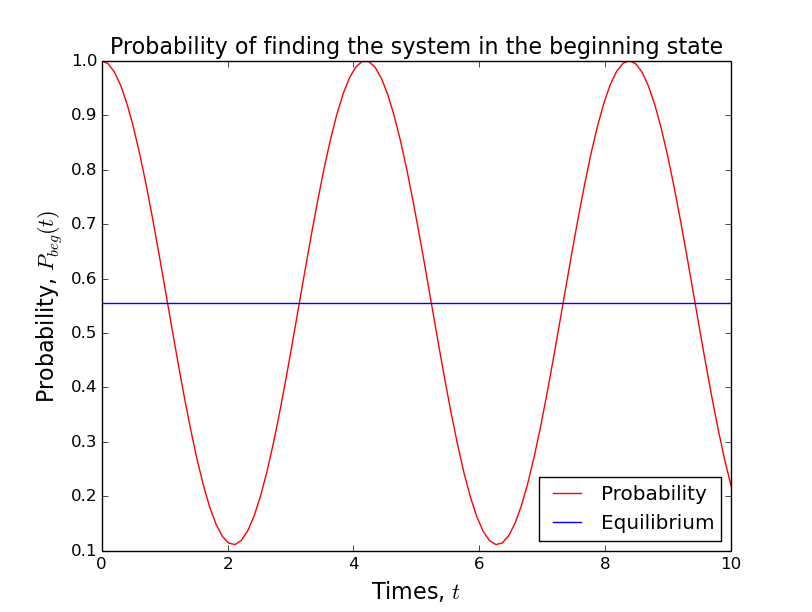
\includegraphics[width=110mm]{figure_1.png}
\caption{Exact versus approximate solution for $n=10$ when we find the second-derivative for the function $f(x)=100e^{-10x}$. \label{overflow}}
\end{figure}
\begin{figure}[!htbp]
\centering
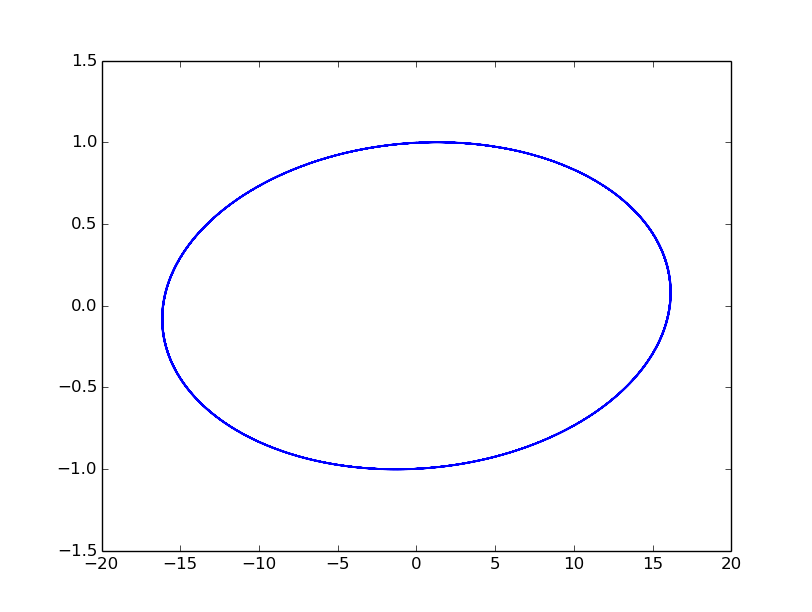
\includegraphics[width=110mm]{figure_2.png}
\caption{Exact versus approximate solution for $n=100$ when we find the second-derivative for the function $f(x)=100e^{-10x}$. \label{overflow}}
\end{figure}
The time was calculated by 'ctime' (see last section of theory), and the result is found in \textit{Table 1}.
\begin{table}[!htbp]
 \centering
 \begin{tabular}{c|c|c|c}
   \toprule
   $n$ & General & Special & LU\\
   \midrule
   $10^1$ & 0.000306 & 0.000803 & 0.001323\\
   $10^2$ & 0.001757 & 0.001669 & 0.002284\\
   $10^3$ & 0.019549 & 0.016393 & 0.077436\\
   $10^4$ & 0.140944 & 0.240213 & 20.5251\\
   $10^5$ & 0.954841 & 2.20564 & --\\
   $10^6$ & 9.46947 & 7.26546 & --\\
   $10^7$ & 94.1885 & 65.0328 & --\\
   \bottomrule
 \end{tabular}
 \caption{This table shows run time for different $n$-values $n\in [10,10^7]$ for the special solver, general solver and LU decomposition.}
 \label{tab:table1}
\end{table}
Here the time has unit seconds.\par\vspace{3mm}
The last results are associated with the relative error, which is calculated with the algorithm found in the Theory part (in my attached code you will find this implemented in a Python script, but the ideas are equal). You can find the maximum error for $n=10^1,\,\,10^2,...,10^7$ in \textit{Table 2} (The approximate solution in this case is calculated by the general solver).
\begin{table}[!htbp]
 \centering
 \begin{tabular}{c|c}
   \toprule
   $n$ & Max. Error\\
   \midrule
   $10^1$ & -1.17969101897\\
   $10^2$ & -3.08630897354\\
   $10^3$ & -4.81538180677\\
   $10^4$ & -5.09296964363\\
   $10^5$ & -5.32406010548\\
   $10^6$ & -5.20433164963\\
   $10^7$ & -5.99978279849\\
   \bottomrule
 \end{tabular}
 \caption{This table shows run time for different $n$-values $n\in [10^1,\,\,10^7]$ for the special solver, general solver and LU decomposition.}
 \label{tab:table2}
\end{table}
I have also decided to attach a figure where I plot the relative error as a function of $log_{10}(h)$ (\textit{see Figure 3}).\par
\begin{figure}[!htbp]
\centering
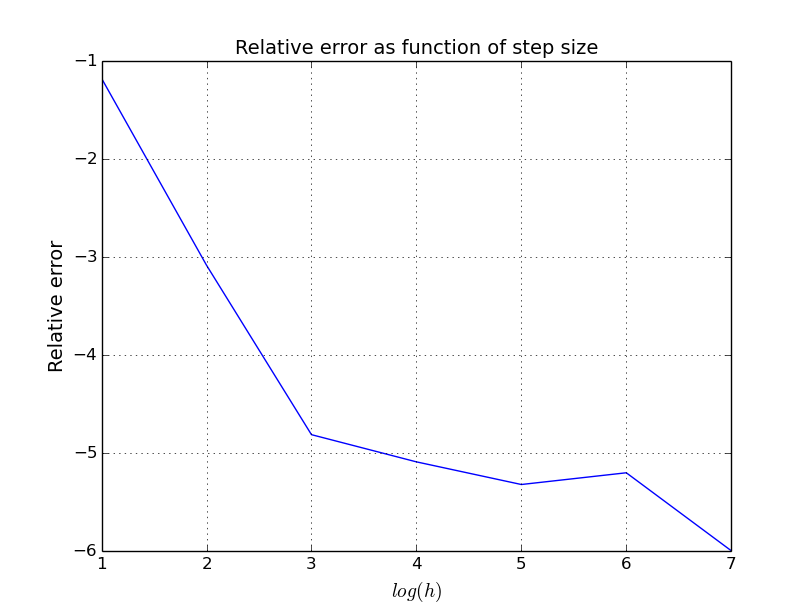
\includegraphics[width=110mm]{figure_4.png}
\caption{Relative error as function of $log(h)$ plotted for $n\in[10^1,\,\,10^7]$.
\label{overflow}}
\end{figure}

\section{Discussion}
From \textit{Figure 1} we can see that the approximate solution is underlying the exact solution, like it should be. When I increase $n$ to $10^3$, we almost cannot see any difference between the approximate and the exact solution. I could added more plots for different values of $n$, but they would look very similar to the two that I have taken with, so i decided to do not (actually I cannot see any difference between $n=1000$ and $n>1000$). This is also why I only used the plots from the general solver - they are similar to the plots from the special solver and the LU decomposition. \par\vspace{3mm}
Something that is not similar between the three methods, is how long time they take. For small vales of $n$ the time difference is not so visible, and the reason is probably that writing of file stands for the major of the time spent. When we increase $n$, the calculations will take over and use the major of time, and therefore we should just compare the results for large $n$'s (when we are interested in the calculation time). As we see, the special algorithm is the fastest, like expected. For $n=10^7$ the special solver takes in fact about $2/3$ of the time of what the general solver takes, and that is exactly what we could expect from the theory part! We also see that the LU decomposition is pretty slow compared with the others, and actually it did not let me run for larger than $n=10^4$. I got this error message (\textit{see Figure 4}):\par
\begin{figure}[!htbp]
\centering
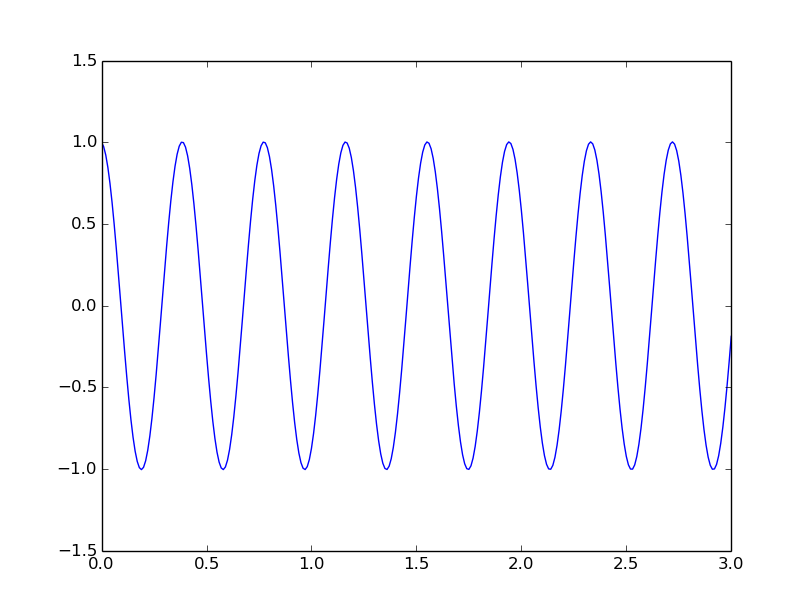
\includegraphics[width=110mm]{figure_3.png}
\caption{The error message when I try to run the LU-depomosition for $n=10^5$ \label{overflow}}
\end{figure}
so the matrix is too big for Armadillo.\par\vspace{3mm}
The relative error is decreasing as smaller the step length is, and that is logical. But what happens from $n=10^5$ to $n=10^6$? The error is actually increasing again! The thing is that the step length $h$ is being so small that truncation error occurs, which happens  because the computer is just able to render a finite number of digits. A standard computer today has a 64-bits processor, which is able to render $\tilde16$ digits. When the numbers are getting really small (I mean, like $10^-6$), we only have 10 significant digits left to express the number. Then the computer has to round off, and we will get truncation errors (so yes, we have errors in the relative error). From $n=10^6$ to $n=10^7$ the error is decreasing again, but that is not logical, so something is wrong in my script (but I cannot find where). This also results that \textit{Figure 3} is wrong. I decided to calculate the error only for the general solver, since the errors are almost the same. The major difference is the GPU time, as we have seen.

\section{Conclusion}
In this project we have seen how we can implement the second derived numerical with different methods. We saw that the GPU time depends on which method we use, and that the calculation time is proportional with the number of FLOPS. We also detected truncation error, and found which $n$ that gives less error. Almost everything worked as expected, the only exception was the maximum error when $n=10^7$. Often we are not so lucky that our result is what it is supposed to be, so I think it was pretty funny. I learned how to find an approximate solution by using linear algebra, and there is always funny when methods work. Of course, writing scripts, debug, understand algorithms - and not least writing rapport takes some time, maybe I will ally with someone on the next project. But all in all for me the project seems to be conducted, and right now I cannot find any improvements.

\section{Bibliography}
\begin{enumerate}
\item "Lecture notes", Morten Hjorth-Jensen (2015)
\end{enumerate}
\end{document}